%!TEX root = alga.tex
\begin{figure*}
\begin{subfigure}[b]{0.2\linewidth}
\centerline{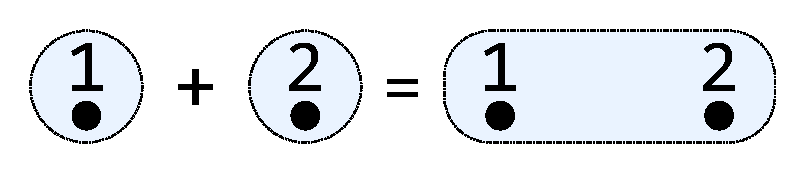
\includegraphics[scale=0.27]{fig/ex-a.pdf}}
\vspace{-2.4mm}
\caption{$1 + 2$}
\centerline{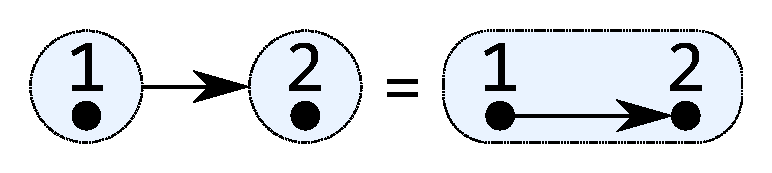
\includegraphics[scale=0.27]{fig/ex-b.pdf}}
\vspace{-2.4mm}
\caption{$1 \rightarrow 2$}
\end{subfigure}
\hspace{11mm}
\begin{subfigure}[b]{0.17\linewidth}
\centerline{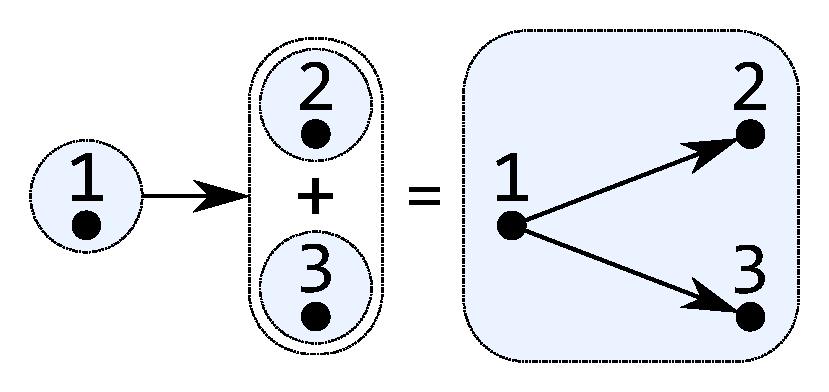
\includegraphics[scale=0.27]{fig/ex-c.pdf}}
\vspace{-1mm}
\caption{$1 \rightarrow (2 + 3)$}
\end{subfigure}
\hspace{12mm}
\begin{subfigure}[b]{0.15\linewidth}
\centerline{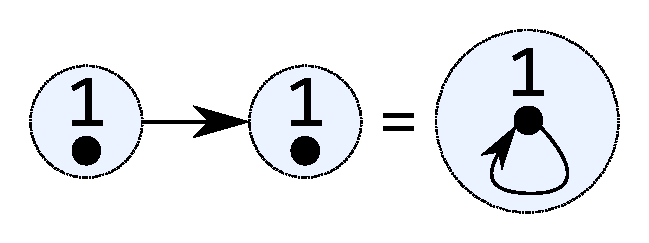
\includegraphics[scale=0.27]{fig/ex-d.pdf}}
\vspace{2.4mm}
\caption{$1 \rightarrow 1$}
\end{subfigure}
\hspace{12mm}
\begin{subfigure}[b]{0.2\linewidth}
\centerline{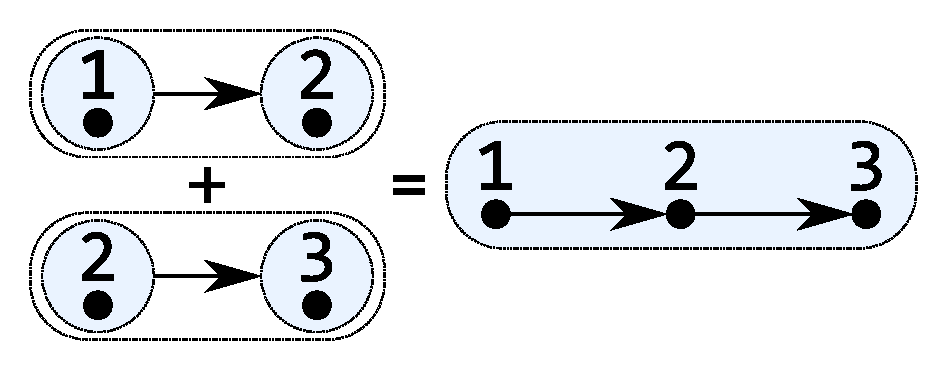
\includegraphics[scale=0.27]{fig/ex-e-new.pdf}}
\vspace{-1mm}
\caption{$1 \rightarrow 2 + 2 \rightarrow 3$}
\end{subfigure}
\caption{Examples of graph construction. The overlay and connect operations are denoted
by $+$ and $\rightarrow$, respectively.\label{fig-construction}}
\end{figure*}

\section{The core}\label{sec-core}
In this section we define the \emph{core} of algebraic graphs comprising
four graph construction primitives. We describe the semantics of the primitives
using the common representation of graphs by sets of vertices and edges, and
then abstract away from this representation by focusing on the laws that these
primitives satisfy.

Let $G$ be the set of all directed graphs whose vertices come from a fixed
universe $\mathbb{V}$. As an example, we can think of graphs whose vertices are
positive integers. A graph $g \in G$ can be represented by a pair $(V, E)$ where
$V\subseteq \mathbb{V}$ is the set of its vertices and $E \subseteq V \times V$ is
the set of its edges. As mentioned in~\S\ref{sec-intro}, when $E \nsubseteq V \times V$
the pair $(V, E)$ is inconsistent and does not correspond to a graph.

When one needs to guarantee the internal consistency of a data structure, the standard
solution is to define an abstract interface that encapsulates the data structure and
provides a set of safe construction primitives. This is exactly the approach we take.

\subsection{Constructing graphs}\label{sub-constructing}

The simplest possible graph is the \emph{empty} graph. We denote it by
$\varepsilon$, therefore $\varepsilon = (\varnothing, \varnothing)$ and
$\varepsilon \in G$. A graph with a \emph{single vertex} $v \in \mathbb{V}$
is denoted simply by $v$. For example, $1 \in G$ is the graph
$({1}, \varnothing)$.

To construct larger graphs from the above primitives we define binary
operations \emph{overlay} and \emph{connect}, denoted by $+$ and $\rightarrow$,
respectively. The overlay operation $+$ is defined as
\[
(V_1, E_1) + (V_2, E_2)~~\defeq~~(V_1 \cup V_2, E_1 \cup E_2).
\]
That is, the overlay of two graphs comprises the union of their vertices and edges.
The connect $\rightarrow$ operation is defined similarly:
\[
(V_1, E_1) \rightarrow (V_2, E_2)~~\defeq~~(V_1 \cup V_2, E_1 \cup E_2 \cup V_1 \times V_2).
\]
The difference is that when we connect two graphs, an edge is added from each
vertex of the left-hand argument to each vertex of the right-hand
argument\footnote{Our definitions of overlay and connect coincide
with those of graph \emph{union} and \emph{join}, respectively,
e.g see~\citet{1969_graph_theory_harary},
however the arguments of union and join are typically assumed to have disjoint
sets of vertices. We make no such assumptions, hence our definitions are total:
any graphs can be composed using overlay and connect.}.
Note that the connect operation is the only source of edges when constructing
graphs. As we will see in~\S\ref{sec-algebra}, overlay and connect
are very similar to addition and multiplication. We therefore give connect a higher
precedence, i.e. $1 + 2 \rightarrow 3$ is interpreted as $1 + (2 \rightarrow 3)$.
Fig.~\ref{fig-construction} illustrates a few examples of graph construction
using the defined primitives:
\begin{itemize}
  \item $1 + 2$ is the graph with two isolated vertices 1 and 2.
  \item $1 \rightarrow 2$ is the graph with an edge between vertices 1 and 2.
  \item $1 \rightarrow (2 + 3)$ is the graph with three vertices $\{1, 2, 3\}$
  and two edges $(1, 2)$ and $(1, 3)$.
  \item $1 \rightarrow 1$ is the graph with vertex 1 and the \emph{self-loop}.
  \item $1 \rightarrow 2 + 2 \rightarrow 3$ is the graph with three vertices $\{1, 2, 3\}$
  and two edges $(1, 2)$ and $(2, 3)$.
\end{itemize}

As shown in~\S\ref{sec-intro}, the core can be represented by a simple
data type \hs{Graph}, parameterised by the type of vertices~\hs{a}.
To make the core more reusable, the next subsection defines the core type class that
has the usual inhabitants, such as the pair $(V,E)$, data types from
\textsf{containers} and \textsf{fgl}, as well as other, stranger forms of life.

\subsection{Type class}\label{sub-class}

We abstract the graph construction primitives defined in \S\ref{sub-constructing}
as the type class \hs{Graph}\footnote{The name collision (\hs{data Graph}
and \hs{class Graph}) is not a problem in practice, because the data type and type class
are not used together and live in separate modules.}:

\begin{minted}{haskell}
class Graph g where
    type Vertex g
    empty   :: g
    vertex  :: Vertex g -> g
    overlay :: g -> g -> g
    connect :: g -> g -> g
\end{minted}

\noindent
Here the associated type\footnote{Associated
types~\cite{2005_associated_type_chakravarty} require the \textsf{TypeFamilies}
GHC extension.} \hs{Vertex@\,\blk{g}@} corresponds to the universe of graph
vertices $\mathbb{V}$, \hs{empty} is the empty graph
$\varepsilon$, \hs{vertex} constructs a graph with a single vertex,
and \hs{overlay} and \hs{connect} compose given graphs according to
the definitions in~\S\ref{sub-constructing}. All methods of the type class
are total, i.e. are defined for all possible inputs, therefore,
the presented API allows \emph{fewer opportunities for usage errors}
and \emph{greater opportunities for reuse}.

Let us put the interface to the test and construct some graphs. A single edge is
obtained by connecting two vertices:

\begin{minted}{haskell}
edge :: Graph g => Vertex g -> Vertex g -> g
edge x y = connect (vertex x) (vertex y)
\end{minted}

\noindent
The graphs in Fig.~\ref{fig-construction}(b,d) are \hs{edge@\,@1@\,@2} and
\hs{edge@\,@1@\,@1}, respectively.
A graph that contains a given list of isolated vertices can be constructed
as follows:

\begin{minted}{haskell}
vertices :: Graph g => [Vertex g] -> g
vertices = @\std{foldr}@ overlay empty . @\std{map}@ vertex
\end{minted}

\noindent
That is, we turn each vertex into a singleton graph and overlay the results.
The graph in Fig.~\ref{fig-construction}(a) is \hs{vertices@\,@[1,2]}.
By replacing \hs{overlay} with \hs{connect} in the above
definition, we obtain a directed \emph{clique} -- a fully connected graph
on a given list of vertices:

\begin{minted}{haskell}
clique :: Graph g => [Vertex g] -> g
clique = @\std{foldr}@ connect empty . @\std{map}@ vertex
\end{minted}

\noindent
For example, \hs{clique@\,@[1,2,3]} expands to
$1 \rightarrow 2 \rightarrow 3 \rightarrow \varepsilon$, i.e.
the graph with three vertices $\{1, 2, 3\}$ and three edges $(1, 2)$, $(1, 3)$ and
$(2, 3)$. Note that it is different from the graph in Fig.~\ref{fig-construction}(e).

The graph construction functions defined above are total, fully polymorphic, and elegant.
Thanks to the minimalistic core type class, it is easy to wrap your favourite
graph library into the described interface, and reuse the above functions, as
well as many others that we define throughout this paper.
